\documentclass[a4paper, 12pt, twoside]{report}

% ========================
% ======= Imports
% ========================

\usepackage[utf8]{inputenc}             % LaTeX, comprend les accents !
\usepackage[T1]{fontenc}                % Meilleur rendu des accents sur PDF
\usepackage[francais]{babel}            % Typographie française
\usepackage{lmodern}                    % Police Latin Modern
\usepackage{ae,aecompl}                 % Rendu de police amélioré
\usepackage[top=2.5cm, bottom=2cm,      % Définition des marges du document
		left=3cm, right=2.5cm,
		headheight=15pt]{geometry}
\usepackage{graphicx}                   % Insertion d'image
\usepackage{eso-pic}	                % Image d'arrière-plan
\usepackage{array}                      % Amélioration tableaux
\usepackage{hyperref}                   % Liens cliquables sur PDF
\usepackage{lastpage}                   % Numérotation pied de page
\definecolor{bleuleger}{RGB}{0,0,200}   % Couleur personnalisée bleuleger

\usepackage{listings}                   % Affichage de code source
\lstnewenvironment{codeC}[1][]          % Environnement perso pour code C
{%
	\lstset{language=C,
		frame=single,
		captionpos=b, 
		backgroundcolor=\color{bleuleger!5},
		basicstyle=\ttfamily\tiny,
		numbers=left,
		numberstyle=\color{black},
		numbersep=5pt,
		breaklines=true,
		tabsize=4,
		keywordstyle=\bfseries\color{green!40!black},
		stringstyle=\color{red}\ttfamily,
		identifierstyle=\color{blue},
		caption={[#1]{#1}},           
		commentstyle=\color{purple!40!black}}
}
{}

\usepackage[
  backend=biber,
  style=apa,
  sorting=none,
  babel=other
]{biblatex}
\addbibresource{bibliographie.bib}
\addbibresource{webographie.bib}

\usepackage{float} % pour l’option [H]
\usepackage{diagbox}

%%%%%%%%%%%%%%%%%%%%%%%%%%%%%%%%%%%%%%%%%%%%%%%%%%%%%%%%%%%%%%%%%%%%%%%

%%%%%%%%%%%%%%%%%%%%%%%%%%%%%%%%%%%%%%%%
%    Page de garde (Pagedegarde.tex)   %
%%%%%%%%%%%%%%%%%%%%%%%%%%%%%%%%%%%%%%%%
% Dorian Depriester, 2014
\usepackage{fancyhdr}
\usepackage{nomencl}
\makeatletter
\def\@ecole{école}
\newcommand{\ecole}[1]{
  \def\@ecole{#1}
}

\def\@entreprise{École Normale Supérieure (ENS-PSL)}
\newcommand{\entreprise}[1]{
  \def\@entreprise{#1}
}

\def\@datedebut{\today}
\newcommand{\datedebut}[1]{
  \def\@datedebut{#1}
}


\def\@datefin{\today}
\newcommand{\datefin}[1]{
  \def\@datefin{#1}
}


\def\@specialite{Spécialité}
\newcommand{\specialite}[1]{
  \def\@specialite{#1}
}

\def\@ED{\'{E}cole Doctorale}
\newcommand{\ED}[1]{
  \def\@ED{#1}
}

\def\@doctorat{Doctorat}
\newcommand{\doctorat}[1]{
  \def\@doctorat{#1}
}

\def\@adresse{Adresse}
\newcommand{\adresse}[1]{
  \def\@adresse{#1}
}

\def\@directeur{directeur}
\newcommand{\directeur}[1]{
  \def\@directeur{#1}
}

\def\@fonction{Développeur }
\newcommand{\fonction}[1]{
  \def\@fonction{#1}
}

\def\@encadrant{encadrant}
\newcommand{\encadrant}[1]{
  \def\@encadrant{#1}
}
\def\@jurya{}{}{}
\newcommand{\jurya}[3]{
  \def\@jurya{#1,	& #2	& #3\\}
}
\def\@juryb{}{}{}
\newcommand{\juryb}[3]{
  \def\@juryb{#1,	& #2	& #3\\}
}
\def\@juryc{}{}{}
\newcommand{\juryc}[3]{
  \def\@juryc{#1,	& #2	& #3\\}
}

\makeatother

\newcommand\BackgroundPic{%
	\put(0,0){%
		\parbox[b][\paperheight]{\paperwidth}{%
			\includegraphics[height=0.45\paperheight]{images/bordure.png}%
			\vfill
		}
	}
}
\newcommand\EtiquetteThese{%
	\put(0,0){%
		\parbox[t][\paperheight]{\paperwidth}{%
			\hfill
			%\colorbox{blue}{		
				\begin{minipage}[b]{2em}
					
\includegraphics[width=4.0\textwidth]{images/logo_miage.png}\\					
					%\centering\Huge\textcolor{white}{M\\I\\A\\G\\E\\}
					\vspace{0.2cm}
				\end{minipage}
			%}
		}
	}
}

\makeatletter
\newcommand{\pagedegarde}{
\newgeometry{top=2.5cm, bottom=1cm, left=2cm, right=1cm}
\AddToShipoutPicture*{\BackgroundPic}
%\AddToShipoutPicture*{\EtiquetteThese}
  \begin{titlepage}
  \centering
      
\includegraphics[width=0.6\textwidth]{images/logo_Paris_Nanterre_couleur_RVB.png}
      \hfill
      
\includegraphics[width=0.20\textwidth]{images/ens_logo.png}\\
    \vspace{1cm}
     % {\Large Licence MIASHS parcours MIAGE}\\
    \vspace{1cm}
      {\huge 
      	{\bfseries Mémoire de M1}\\
    \vspace{0.5cm}}
      	Master MIAGE (apprentissage)\\
    \vspace{1cm}
   		
    \vspace{1cm}
    	{\huge\color[rgb]{0,0,1} \bfseries{\@title}}\\
    \vspace{0.5cm}
    {\bfseries Entreprise d'accueil : \@entreprise}\\
    {\bfseries Mémoire réalisé du \@datedebut\ au \@datefin}\\
    %	{\Large{\bfseries Spécialité doctorale ``\@specialite''}}\\
    \vspace{2cm}
    	\textit{présenté et soutenu par}\\
    \vspace{0.5cm}
    	{\Large {\bfseries \@author}} \\
    \vspace{0.5cm}
    	le \@date \\
    \vfill
	\begin{tabular}{>{\bfseries}lll}
		\large Jury de la soutenance\\
		\vspace{0.15cm}\\
		\@jurya
		\@juryb
		\@juryc
	\end{tabular}
	\vfill
  \end{titlepage}

\restoregeometry  
\makenomenclature

\pagestyle{fancy}

\renewcommand\headrulewidth{1pt}

\fancyhead[L]{\@fonction}

\fancyhead[R]{\@entreprise}


\renewcommand\footrulewidth{1pt}

\fancyfoot[L]{\@author}

\fancyfoot[C]{}

\fancyfoot[R]{ Page \thepage/\pageref{LastPage}}
}


%%%%%%%%%%%%%%%%%%%%%%%%%%%%%%%%%%%%%%%%%%%%%%%%%%%%%%%%%%%%%%%%%%%%%%%


% ========================
% == Début du document
% ========================

\begin{document}

%%%%%%%%%%%%%%%%%%%%%%%%%%%%%%%%%%%%%%%%%%%%%%%%%%%%%%%%%%%%%%%%%%%%%%%

% ========================
% ==== Page de garde
% ========================

\author{Kevin SOARES}
\title{Les agents IA dans la réalisation de projets  de développement}
\entreprise{École Normale Supérieure (ENS - PSL)}
\fonction{Apprenti SIFAC}
\datedebut{2 septembre 2024}
\datefin{28 mai 2025}

\date{10 juin 2025}

\jurya{M. François DELBOT}{Maître de conférences}{Responsable du master / Tuteur}
\juryc{M. Stéphane POULAIN}{Directeur Financier}{Maître d'apprentissage}

\pagedegarde

%%%%%%%%%%%%%%%%%%%%%%%%%%%%%%%%%%%%%%%%%%%%%%%%%%%%%%%%%%%%%%%%%%%%%%%

% ========================
% ==== Remerciements 
% ========================

\chapter*{Remerciements}

Je tiens tout d’abord à exprimer ma sincère gratitude à \textbf{M.~François Delbot}, Maître de conférences et responsable du Master, pour son accompagnement tout au long de mon parcours. Déjà tuteur enseignant lors de mon stage de fin d’année précédente, il m’a de nouveau soutenu cette année, en m’aidant à définir une problématique pertinente pour ce mémoire. Je le remercie chaleureusement pour son engagement constant et la qualité de son encadrement.

Mes remerciements vont également à \textbf{M.~Karim El-Mahou}, qui a été mon tuteur lors mon arrivée à l’ENS. Son soutien technique comme humain a grandement facilité mon intégration et orienté mes premiers travaux.

Je souhaite enfin remercier \textbf{M.~Stéphane Poulain}, directeur du département, pour l’accueil chaleureux qu’il m’a réservé et pour les conditions de travail qu’il a mises en place. Sa disponibilité et ses conseils avisés ont contribué à faire de cette expérience un moment riche tant sur le plan professionnel que personnel.




%%%%%%%%%%%%%%%%%%%%%%%%%%%%%%%%%%%%%%%%%%%%%%%%%%%%%%%%%%%%%%%%%%%%%%%

% ========================
% ==== Resumé
% ========================

\chapter*{Résumés ($1$ page)}
\section*{Résumé}
Les progrès récents des Large Language Models (LLMs) et des architectures multi-agents soulèvent une question audacieuse : peut-on remplacer une équipe de développement logicielle par un collectif d’agents IA ?  Afin d’éclairer ce débat, ce mémoire dresse d’abord l’état de l’art des LLMs appliqués au génie logiciel, puis cartographie les fonctions clés, de l’analyse d’exigences à la mise en production, qu’une équipe doit assumer.  L’examen de trois prototypes représentatifs (\textit{CodePori}, \textit{Agent-Driven Automatic Software Improvement} et un pipeline Auto-DevOps multi-agents) montre que la génération, les tests et le débogage peuvent déjà être automatisés avec un taux de précision compris entre 80 et 90\%.  Cependant, les risques de biais, d’hallucinations et de fuites de données obligent à maintenir des garde-fous et une supervision humaine, notamment pour l’architecture et la gouvernance.  Une matrice SWOT met en évidence des forces (exécution 24 / 7, coûts réduits), mais aussi des menaces (responsabilité légale, attaques backdoor).  Trois scénarios d’évolution sont proposés : \emph{développement assisté} à court terme, \emph{équipes hybrides} à moyen terme, puis \emph{autonomie quasi complète} sous audits périodiques.  La conclusion affirme que le remplacement total est techniquement concevable, mais conditionné à l’alignement, à la sécurité et à un cadre réglementaire robuste.  Ce travail offre ainsi un outil d’aide à la décision pour chercheurs, industriels et législateurs confrontés à l’émergence des équipes 100\% IA.

\section*{Abstract}
Recent advances in \emph{Large Language Models} (LLMs) and multi-agent systems raise a bold question: can a software development team be entirely replaced by AI agents?  To address this, the thesis first surveys state-of-the-art LLM techniques for software engineering and maps essential roles, from requirements analysis to production deployment, that any team must cover.  Three representative prototypes (\textit{CodePori}, \textit{Agent-Driven Automatic Software Improvement}, and an Auto-DevOps multi-agent pipeline) reveal that code generation, testing and debugging can already be automated with 80 to 90\% accuracy.  Yet bias, hallucinations and data-leak risks still demand human oversight for architecture and governance.  A SWOT matrix highlights strengths (24 / 7 execution, lower recurring costs) and threats (legal accountability, backdoor attacks).  Building on this analysis, three evolution scenarios are outlined: \emph{AI-assisted pair programming} in the short term, \emph{lean hybrid teams} mid-term, and near-full autonomy under periodic audits in the long run.  The thesis concludes that full replacement is technically plausible but contingent upon reliable alignment, strong security guarantees and a clear regulatory framework.  Overall, the work provides a decision-making tool for researchers, practitioners and policymakers facing the rise of “all-AI” development teams.


%%%%%%%%%%%%%%%%%%%%%%%%%%%%%%%%%%%%%%%%%%%%%%%%%%%%%%%%%%%%%%%%%%%%%%%

\tableofcontents

%%%%%%%%%%%%%%%%%%%%%%%%%%%%%%%%%%%%%%%%%%%%%%%%%%%%%%%%%%%%%%%%%%%%%%%

% ========================
% ==== Introduction
% ========================

\chapter{Introduction}

L’essor des modèles de langage de grande taille (\textbf{Large Language Models} ou LLMs) a bouleversé la façon dont nous interagissons avec le texte : un simple prompt suffit désormais à générer une page de prose, un résumé d’article ou, plus surprenant encore, un extrait de code compilable.  Dans la foulée, une nouvelle génération d’agents IA, capables de raisonner sur plusieurs tours, d’appeler des outils externes et de \textbf{collaborer entre eux}, prétend couvrir l’ensemble du cycle logiciel : rédaction des spécifications, écriture des tests, production du code, déploiement continu.  Face à ces annonces, une question surgit : \textbf{Une équipe de développement peut-elle, à terme, être remplacée entièrement par des agents IA ?}

Ce mémoire propose de répondre à cette interrogation en adoptant une démarche bibliographique structurée.  Nous passons d’abord en revue les principes des LLMs et les architectures multi-agents, puis nous confrontons leurs performances à des benchmarks de génération de code.  Nous analysons ensuite trois prototypes représentatifs : \textit{CodePori}, \textit{Agent-Driven Automatic Software Improvement} et un pipeline Auto-DevOps multi-agents, qui illustrent le potentiel, mais aussi les limites, d’équipes 100 \% IA (ou presque). Enfin, nous synthétisons ces observations via une matrice SWOT et nous esquissons trois scénarios d’évolution, de la programmation assistée d’aujourd’hui à l’autonomie (quasi) complète de demain.

La contribution essentielle de ce travail est double.  D’une part, il offre une \textbf{cartographie des tâches} qu’une équipe de développement doit couvrir et un état de la couverture actuelle par les agents IA.  D’autre part, il identifie les \textbf{conditions critiques} (alignement, sécurité, gouvernance) sans lesquelles le remplacement total demeurerait théorique.  L’objectif n’est pas de trancher définitivement, mais de fournir au lecteur une grille d’analyse argumentée pour évaluer la faisabilité, les risques et les opportunités d’un tel bouleversement.

Le plan suit une logique progressive : après l’état de l’art \ref{chapitre:etatArtLLM} et l’étude de la dynamique équipe humaine/agents \ref{chapitre:humainAgent}, nous passons aux cas d’usage concrets \ref{chapitre:etudeCas}, puis à une discussion de faisabilité et de perspectives \ref{chapitre:faisabilite}.  La conclusion \ref{conclusion} revient sur les points clés et ouvre sur les recherches futures, qu’elles soient techniques, organisationnelles ou éthiques.

En somme, ce mémoire vise à montrer pourquoi le sujet est crucial, comment nous l’avons abordé, et en quoi nos résultats peuvent éclairer décideurs, chercheurs et praticiens.  Le lecteur n’a pas besoin d’être expert en IA : il trouvera ici les repères nécessaires pour comprendre les promesses, les limites et les implications d’une \textbf{éventuelle équipe de développement sans développeurs}.


%%%%%%%%%%%%%%%%%%%%%%%%%%%%%%%%%%%%%%%%%%%%%%%%%%%%%%%%%%%%%%%%%%%%%%%

% ========================
% ==== Méthodologie
% ========================

\chapter{Méthodologie}

\section{Systematic Mapping Study (SMS)}

La \textbf{Systematic Mapping Study} (SMS) est une méthode de revue de littérature formelle visant à cartographier et classer l’état de l’art d’un domaine de recherche de façon exhaustive et reproductible. Elle se déroule en quatre grandes phases :

\begin{enumerate}
  \item \textbf{Définition des questions de recherche} (QR) et des objectifs de la carte ;
  \item \textbf{Recherche systématique} des publications pertinentes dans les bases de données (ex. IEEE Xplore, Scholar, ACM) selon des chaînes de requêtes préétablies ;
  \item \textbf{Sélection et filtrage} des articles via des critères d’inclusion/exclusion, combinant filtrage automatique (titres, abstracts, scoring) puis examen manuel (abstract, introduction, table des matières, conclusion) ;
  \item \textbf{Classification et synthèse} des résultats : attribution de catégories thématiques, visualisation sous forme de matrice ou de graphique, identification des lacunes et des tendances.
\end{enumerate}

Dans ce mémoire, nous appliquons la démarche SMS pour structurer notre recherche bibliographique sur la génération automatique de code par agents IA. Chaque étape (définition des requêtes, filtrage, scoring, classification) suit le protocole SMS afin d'assurer fiabilité, transparence et reproductibilité des travaux existants.


\section{Méthode PICO}

Pour structurer la question de recherche, nous utilisons la méthode \textbf{PICO}.
Cette approche, acronyme de 
\textit{Population}, \textit{Intervention}, \textit{Comparison} et \textit{Outcomes},
exige de définir explicitement ces quatre composantes. Elle aide ainsi à formuler une question précise et à guider la recherche .

Notre question de recherche est formulée de la manière suivante : "Est-il possible de remplacer entièrement une équipe de développement par des agents IA ?"

Le tableau \ref{PICO} présente la décomposition de notre problématique selon la méthode PICO.

\begin{table}[H]
\centering
\begin{tabular}{|p{4cm}|p{9cm}|}
  \hline
  \textbf{Élément} & \textbf{Application au mémoire} \\
  \hline
  \textbf{P}opulation & Équipe de développement \\
  \hline
  \textbf{I}ntervention & Remplacement par des agents IA \\
  \hline
  \textbf{C}omparison & Équipe humaine traditionnelle \\
  \hline
  \textbf{O}utcomes & Faisabilité technique d’un remplacement total \\
  \hline
\end{tabular}
\caption{Formulation PICO de la question de recherche}
\label{PICO}
\end{table}

\section{Formulation des requêtes}

La méthode PICO décrite ci-dessus nous permet ainsi de formuler les requêtes nous permettant d'interroger les bases de données scientifiques et de pouvoir en extraire des papiers utiles à notre recherche. Pour répondre à celle-ci, nous divisons notre recherche en quatre requêtes :

\begin{itemize}
    \item Définition de LLM
    \item Définition d'agent IA
    \item Taille et composition idéales d'une équipe de développement
    \item Remplacement d'une équipe de développement par des agents IA
\end{itemize}

Ces quatre requêtes vont nous permettre de définir ce que sont des LLM ainsi que des agents IA, pour ensuite examiner les papiers consacrés à la taille et composition idéales d'une équipe. Enfin, nous explorerons les travaux sur la génération automatique de code par les agents IA ce qui nous fournira les éléments nécessaires pour croiser ces informations et déterminer dans quelle mesure une équipe humaine peut ou non être remplacée par des agents IA.

Pour la recherche, nous utilisons Google Scholar qui permet de chercher des papiers dans différentes bases (e.g. IEEE ou ArXiv) ce qui en fait l'outil le plus polyvalent pour nos besoins.

\subsection{Définition de LLM}

Cette requête (Listing 2.1) nous met à disposition les papiers permettant de définir le terme "LLM".

\begin{codeC}[Requête - LLM]

    allintitle:"large language model" ("systematic literature review" OR survey OR taxonomy)
\end{codeC}

\subsection{Définition d'Agents IA}

Cette requête (Listing 2.2) recense les papiers proposant des définitions d’agents IA (ou " LLM agents "), afin de cerner précisément ce concept.

\begin{codeC}[Requête - Agents IA]
    allintitle:(agent OR "LLM agent") (taxonomy OR definition)
\end{codeC}

\subsection{Taille et composition idéales d'une équipe de développement}

Cette requête (Listing 2.3) vise la littérature traitant de la taille idéale et de la composition optimale des équipes de développement logiciel.

\begin{codeC}[Requête - Equipe de développement]
    intitle:"team size" AND ideal AND (software development OR agile OR scrum)
\end{codeC}

\subsection{Remplacement d'une équipe de développement par des Agents IA}

Cette requête (Listing 2.4) rassemble les travaux étudiant dans quelle mesure des agents IA sont capables de générer automatiquement du code et peuvent remplacer une équipe de développement humaine.

\begin{codeC}[Requête - Remplacement équipe de développement]
    ("automatic code generation" OR "code synthesis" OR "AI-generated code") AND (intitle:agent OR intitle:"software agent" OR intitle:"AI agent")
\end{codeC}

\section{Filtrage}

Avant de lire entièrement chaque papier, nous appliquons plusieurs étapes de filtrage afin de conserver uniquement les papiers essentiels et qui auront une réelle utilité au développement de nos propos.

\subsection{Filtrage sur l'année}
Notre premier critère de filtrage, appliqué directement lors de la recherche depuis Google Scholar, est l'année.

Pour chaque recherche, un filtre sur l'année a été appliqué :
Pour la définition de LLM  (Listing 2.1) et l'automatisation du développement avec agents IA (Listing 2.4) nous recherchons uniquement les papiers publiés à partir de 2024. Ce choix est dû au grand nombre de papiers traitant des LLM et à l'essor récent de ceux-ci ces dernières années, cela nous permet donc premièrement de retenir moins de papiers et deuxièmement d'avoir des études plus récentes et actuelles de ceux-ci. On passe donc de 121 à 101 papiers pour la définition des LLM et de 325 à 63 papiers pour l'automatisation du développement avec agents IA.

Concernant la définition des agents IA (Listing 2.2) et la composition et taille idéales d'une équipe de développement (Listing 2.3) nous recherchons uniquement les papiers publiés à partir de 2024. On passe donc de 174 à 22 papiers pour la définition des agents IA et de 127 à 30 papiers pour l'équipe de développement.

\subsection{Filtrage sur le type de document}

Après extraction des différents papiers à l'aide de Zotero, nous commençons les étapes de filtrage plus précises passant par différents scripts python. La première d'entre elles est un filtrage sur le type de document.
Nous pouvons voir dans nos papiers différents types de documents, en voici la liste exhaustive ainsi que leur nombre :

\begin{itemize}
    \item journalArticle : 108
    \item preprint : 66
    \item conferencePaper : 28
    \item bookSection : 7
    \item thesis : 3
    \item document : 2
    \item report : 1
    \item book : 1
\end{itemize}

Nous décidons donc d'exclure les papiers de type \textit{report} et \textit{document} étant des types de documents sans description ne nous permettant pas de savoir au premier abord de quel papier il s'agit.
Le tableau \ref{filtrageTypeDoc} montre le nombre de papiers pour chaque requête avant et après le filtrage sur le type de document.

\begin{table}[H]
\centering
\begin{tabular}{|c|c|c|}
  \hline
  \textbf{Requête} & \textbf{Papiers avant filtrage} & \textbf{Papiers après filtrage}\\
  \hline
  Définition LLMs & 101 & 101 \\
  \hline
  Définition agents IA & 22 & 21 \\
  \hline
  Taille et composition d'équipe & 30 & 29 \\
  \hline
  Automatisation par Agents IA & 63 & 62 \\
  \hline
  \textbf{Total} & 216 & 213 \\
  \hline
\end{tabular}
\caption{Filtrage sur le type de document}
\label{filtrageTypeDoc}
\end{table}

\subsection{Filtrage sur le titre}

Nous continuons le filtrage en procédant à une sélection sur le titre avec une liste de mots éliminatoires tels que 'political', 'philosophy' ou encore 'religion' (une liste exhaustive est disponible en annexe \ref{annexe:mots_eliminatoires}).

Le tableau \ref{filtrageTitre} montre le nombre de papiers pour chaque requête avant et après filtrage sur le titre.

\begin{table}[H]
\centering
\begin{tabular}{|c|c|c|}
  \hline
  \textbf{Requête} & \textbf{Papiers avant filtrage} & \textbf{Papiers après filtrage}\\
  \hline
  Définition LLMs & 101 & 98 \\
  \hline
  Définition agents IA & 21 & 21 \\
  \hline
  Taille et composition d'équipe & 29 & 26 \\
  \hline
  Automatisation par Agents IA & 62 & 62 \\
  \hline
  \textbf{Total} & 213 & 207 \\
  \hline
\end{tabular}
\caption{Filtrage sur le titre : mots éliminatoires}
\label{filtrageTitre}
\end{table}

\subsection{Filtrage sur l'abstract}

Notre dernière étape de filtrage \textit{"automatique"}, avant le filtrage manuel, sera un système de points sur l'abstract. Pour cela, on établit un système à points qui sont attribués lorsque les mots d'un groupe de mots prédéfini sont présents dans l'abstract. Le maximum étant de 3 points si tous les termes sont compris dans l'abstract et le minimum de 0, si aucun terme n'est présent.
Le tableau \ref{filtrageAbstractScoring} présente pour chaque requête la répartition des papiers en fonction de leur score d’abstract.

\begin{table}[H]
\centering
\begin{tabular}{|c|c|c|c|c|}
  \hline
   \diagbox{\textbf{Requête}}{\textbf{Score}} & \textbf{3pts} & \textbf{2pts} & \textbf{1pts} & \textbf{0pts}\\
  \hline
  Définition LLMs & 5 & 54 & 29 & 10 \\
  \hline
  Définition agents IA & 5 & 3 & 6 & 7 \\
  \hline
  Taille et composition d'équipe & 2 & 13 & 10 & 1 \\
  \hline
  Automatisation par Agents IA & 1 & 5 & 26 & 30 \\
  \hline
  \textbf{Total} & \textbf{14} & \textbf{76} & \textbf{71} & \textbf{48} \\
  \hline
\end{tabular}
\caption{Filtrage sur l'abstract : score}
\label{filtrageAbstractScoring}
\end{table}

Suite aux résultats de ce filtrage, nous garderons les papiers ayant obtenu un score de 3 points. Cependant, nous prenons la décision de garder également ceux ayant obtenu 2 points pour les requêtes \textit{Taille et composition d'équipe} et \textit{Automatisation par Agents IA}.

Il nous reste ainsi un total de 31 papiers à trier manuellement.

\subsection{Filtrage manuel}

Les étapes de filtrage \textit{"automatiques"} sont utiles grâce à leur simplicité et rapidité d'exécution, surtout sur de gros volumes de papiers, mais restent cependant assez limitées au niveau de la compréhension du texte. Nous devons donc procéder à un filtrage manuel en lisant d'abord l'abstract (première étape), puis en passant en revue l'introduction, les titres de sections et la conclusion (deuxième étape) des articles sélectionnés à l'étape précédente.

Le tableau \ref{filtrageManuel} présente le nombre de papiers obtenus après chaque étape de filtrage manuel.

\begin{table}[H]
\centering
\begin{tabular}{|c|c|c|c|}
    \hline
    \textbf{Requêtes} & \textbf{Nombre initial de papiers} & \textbf{1ère étape} & \textbf{2e étape} \\
    \hline
     Définition LLMs & 5 & 2 & \textbf{2}\\
     \hline
     Définition agents IA & 5 & 2 & \textbf{2}\\
     \hline
     Taille et composition d'équipe & 15 & 2 & \textbf{2}\\
    \hline
     Automatisation par Agents IA & 6 & 6 & \textbf{6}\\
     \hline
     \textbf{Total} & \textbf{31} & \textbf{12} & \textbf{12} \\
     \hline
\end{tabular}
\caption{Filtrage manuel}
\label{filtrageManuel}
\end{table}

Nous conservons donc pour notre recherche un total de \textbf{12} papiers dont :
\begin{itemize}
    \item \textbf{2} pour la définition des LLM ;
    \item \textbf{2} pour la définition des agents IA ;
    \item \textbf{2} pour la taille et la composition d’équipe ;
    \item \textbf{6} pour l’automatisation par Agents IA.
\end{itemize}
Évidemment, bien que chaque article soit rattaché à une catégorie ou à une question de recherche précise, les informations qu’il contient peuvent être mobilisées dans différentes parties de ce mémoire.

%%%%%%%%%%%%%%%%%%%%%%%%%%%%%%%%%%%%%%%%%%%%%%%%%%%%%%%%%%%%%%%%%%%%%%%

% ========================
% ==== État de l'art LLMs
% ========================

\chapter{État de l'art des LLMs appliqués au développement informatique} \label{chapitre:etatArtLLM}

\section{Définitions fondamentales : IA, LLM et Agent IA}

\subsection{Intelligence artificielle (IA)}
L’\textbf{intelligence artificielle} (\textbf{IA}) est un domaine de l’informatique visant à concevoir des programmes capables de comprendre leur environnement, raisonner et agir de façon à maximiser la réussite d’objectifs (tels que la reconnaissance d’images, la planification de trajectoires ou, comme dans ce mémoire : \textbf{la génération de code}).

\subsection{Large Language Model (LLM)}
Un \textbf{Large Language Model} (\textbf{LLM}) est un réseau de neurones de type transformeur entraîné sur une large gamme de données. \parencite{cui_risk_2024}. Son objectif est d’estimer la probabilité du prochain mot afin de générer du texte cohérent. Inclure du code source dans le corpus permet au modèle de créer, compléter ou modifier des programmes informatiques. Le LLM est donc essentiellement une "brique" de génération et de raisonnement probabiliste : il produit du \textbf{texte} mais n’interagit pas par lui‑même avec un environnement logiciel.

% cui_risk2024
% "Large language models (LLMs) are the LMs that have billions or even more model parameters pre-trained on massive data, such as LLaMA … and GPT families (e.g., GPT-3, GPT-3.5, and GPT-4). Recently, researchers discovered the scaling law, i.e., increasing the sizes of pre-training data and model parameters can significantly enhance an LM’s capacity for downstream tasks."
%

\subsection{Agent IA}
Nous appelons \textbf{Agent IA} une entité logicielle semi‑autonome voire autonome qui observe un état (par exemple un dépôt git / un projet ou un rapport de tests), planifie une séquence d’actions et exécute ces actions pour atteindre un objectif.  Un agent IA s’appuie sur un ou plusieurs LLMs pour la génération ou la prise de décision et a donc un certain set de compétences, un rôle défini et une mémoire qui lui est propre \parencite{handler_taxonomy_2023}, mais entoure ceci d’une logique d’orchestration : mémoire de travail, appels d’API, exécution de tests, boucles de rétroaction.

% handler_taxonomy_2023
% Each agent is endowed with a unique set of competencies, which include a clearly defined role, an individual memory, as well as access to further contextual resources, such as data, tools, or foundation models… The backbone of their reasoning and interpretative capabilities is rooted in the incorporation of large language models (LLMs)
%
% rasheed_codepori_2024
% Agents are LLM instances, customized to carry out multiple specific tasks, replacing human workflows
%

\subsection{Différences essentielles entre IA, LLM et Agent IA}
Maintenant que nous avons défini ces 3 termes, nous pouvons aborder les différences essentielles entre ceux-ci :

\begin{itemize}
  \item \textbf{Périmètre :} l'IA est l’ensemble. Le LLM est un sous‑ensemble spécialisé dans la modélisation du langage naturel entraîné sur des ensembles de données. L'agent IA est un système logiciel qui intègre potentiellement un ou plusieurs LLMs tout en y ajoutant une couche d’autonomie (planification, action, raisonnement) \parencite{cui_risk_2024}.

% cui_risk_2024
% figure 1 page 1 ("training data")
  
  \item \textbf{Architecture :} le LLM est un modèle de type transformeur ne conservant pas d’état externe entre les appels, tandis que l’agent IA maintient un état persistant et une mémoire de long terme pour effectuer plusieurs tours d’itération \parencite{handler_taxonomy_2023}.

% handler_taxonomy_2023
%Each agent is endowed with a unique set of competencies, which include a clearly defined role and an individual memory.
%
  \item \textbf{Entrées/Sorties :} le LLM prend un prompt textuel et retourne du texte.  L’agent IA accepte des objectifs de haut niveau, invoque des outils (exécution de tests, CI/CD, IDE) et valide les résultats avant de produire un livrable logiciel \parencite{rasheed_codepori_2024}.
  
  \item \textbf{Responsabilité :} un LLM ne porte pas d’intention propre ; toute responsabilité incombe à l’utilisateur.  L’agent IA en revanche inclut une couche de prise de décision et d’alignement dont la sûreté doit être évaluée \parencite{cui_risk_2024}.
\end{itemize}
\noindent En résumé, le LLM est le moteur de génération et de raisonnement, tandis que l’agent IA en est le conducteur capable d’exploiter ce moteur pour naviguer, de manière semi‑autonome / autonome, dans le cycle de vie de l'atteinte de l'objectif défini (dans notre cas : pour le développement logiciel).

\section{Capacités actuelles des LLMs pour la génération de code}

Les benchmarks de complétion et de correction sur code ont rapidement servi d’indicateurs clés pour évaluer les LLMs.
Par exemple, \textbf{HumanEval} (par OpenAI) : \textcite{rasheed_codepori_2024} rapportent que \emph{CodePori}, un système d’agents LLM dont nous ferons l'étude de cas au Chapitre \ref{etudeCodePori}, atteint jusqu’à 89\% d'amélioration de précision du code comparé à une dizaine de modèles de génération de code sur ce benchmark et 85\% lors d’une évaluation manuelle de projets complexes.    

Au-delà des scores, la qualité du code généré (lisibilité, absence de bugs) s’améliore lorsqu’on applique des cycles itératifs d’exécution de tests et de correction automatique :  
\begin{itemize}
  \item Dans \textcite{vallecillos_ruiz_agent-driven_2024}, des agents LLM orchestrés en pipeline [génération → tests → amélioration] démontrent une réduction significative des erreurs "last-mile" (problème présents lors du fin de processus de distribution) grâce à l’apprentissage par rétroaction.  
  %vallecillos_ruiz_agent-driven_2024
  %The iterative nature of agents, which allows for continuous learning and adaptation, can help surpass common challenges in code generation.
  %One distinct challenge is the last-mile problems, errors at the final stage of producing functionally and contextually relevant code.
  %
  \item \textcite{zahid_multi-agent_2024} montrent enfin que la collaboration de plusieurs LLMs spécialisés ("boilerplate writer", "doc generator") réduit le temps de développement et augmente la couverture de tests dans des scénarios de projet réels.  
  %zahid_multi-agent_2024
  %the role of autonomous LLMs in multi-agent AI collaboration, focusing on their impact  on code generation, debugging, project management, and software lifecycle optimization.
  %By automating repetitive tasks, such as writing  boilerplate code and generating documentation, these AI agents reduce developer workload and  enhance productivity.
\end{itemize}


\section{Architectures multi-agents basées LLM}

Les architectures multi-agents tirent parti de plusieurs LLMs collaborant selon des rôles et des topologies variées pour accomplir des tâches complexes de génération de code. 

% Les architectures multi-agents pilotées par des LLM peuvent se caractériser selon plusieurs dimensions principales, telles que proposées par \textcite{handler_taxonomy_2023} :


% handler_taxonomy_2023
% This paper proposes a comprehensive multi-dimensional taxonomy, engineered to analyze how autonomous LLM-powered multi-agent systems balance the dynamic interplay between autonomy and alignment across various aspects inherent to architectural viewpoints such as goal-driven task management, agent composition, multi-agent collaboration, and context interaction.
%

\begin{itemize}
  \item \textbf{Dimension composition d’agents} : \\
    Chaque agent se spécialise dans un sous-ensemble de fonctions (par exemple, analyse des spécifications, génération de code, tests, relecture) et possède sa propre mémoire et accès à des outils externes \parencite{handler_taxonomy_2023}.
% handler_taxonomy_2023
%Each agent is endowed with a unique set of competencies, which include a clearly defined role and an individual memory.
%
    
\item \textbf{Modes de collaboration} :
  \begin{itemize}
    \item Pipeline itératif : les agents s’enchaînent selon un flux génération → tests → amélioration, exploitant les boucles de rétroaction pour corriger par exemple les "last-mile" problems \parencite{vallecillos_ruiz_agent-driven_2024}.
    \item Collaboration distribuée : plusieurs agents LLM, spécialisés (boilerplate writer, doc generator), travaillent en parallèle et consolident leurs résultats pour produire un livrable cohérent \parencite{zahid_multi-agent_2024}.
  \end{itemize}


  \item \textbf{Équilibrage de charge et orchestration} : \\
    Pour optimiser la performance et la cohérence, des stratégies dynamiques redistribuent les tâches entre agents selon la charge actuelle et leur spécialisation  tout en veillant à la convergence des résultats \parencite{handler_balancing_2023}.

  \item \textbf{Niveaux d’autonomie} : \\
    Chaque agent peut opérer de manière plus ou moins autonome selon le degré de supervision humaine et les guardrails définis de l’exécution strictement guidée à l’initiative complète sur des sous-tâches \parencite{handler_taxonomy_2023}.
\end{itemize}

\section{Limites techniques et risques inhérents}

L’utilisation de LLMs et d’agents IA soulève plusieurs enjeux critiques pouvant compromettre la fiabilité, la sécurité et la maintenabilité des solutions logicielles.

\subsection{Biais et hallucinations}
Les LLMs, entraînés sur des jeux de données massifs, intègrent souvent des biais socio-culturels ou sectoriels. Ces biais peuvent conduire à des généralisations inappropriées ou à des décisions discriminatoires dans le code produit. De plus, les modèles peuvent \textbf{halluciner} : générer du code incorrect ou non compilable, voire dangereux (plus généralement, \cite{wikiHallucinationIA} : générer des réponses fausses à partir de modèles ou données inexistantes ) \parencite{cui_risk_2024}.

% cui_risk_2024
% Even without adversarial attacks, current LLMs may still generate untruthful, toxic, biased, and even illegal contents
%

\subsection{Sécurité et confidentialité}
Les processus de formation et d’utilisation des LLMs exposent à des menaces spécifiques tant au niveau de la sécurité que de la confidentialité :
\begin{itemize}
  \item \textbf{Vulnérabilités induites} : du code généré pourrait comporter des backdoors ou exploiter des librairies vulnérables, ouvrant la porte à des attaques ciblées, comme indiqué dans la taxonomy des menaces de \parencite{wang_unique_2024}.

  \item \textbf{Fuite de données sensibles} : les LLMs peuvent mémoriser et régurgiter des extraits de leur corpus d’entraînement, y compris des secrets de configuration ou des clés d’API accidentellement indexées.
\end{itemize}

  % wang_unique_2024
  % This tendency allows adversaries to extract private information. For example, Carlini et al. [13] found that prompts with specific prefixes could cause GPT-2 to generate content containing personal information, such as email addresses and phone numbers.
  % Moreover, malicious third parties involved in developing LLMs in outsourcing scenarios can compromise these models’ integrity and utility through poisoning attacks [168] and backdoor attacks [132]. For example, an attacker could implant a backdoor in an LLM-based automated customer service system
  %

\section{Conclusion}

Nous avons défini les briques fondamentales — IA, LLM et Agent IA — et exploré les capacités actuelles des LLMs pour la génération de code, ainsi que les architectures multi-agents et leurs limites techniques.  
Avant de passer à l’analyse comparative IA vs humain, il est utile de préciser deux critères clés d’évaluation :

\begin{itemize}
  \item \textbf{Degré d’autonomie} : capacité d’un agent à planifier et exécuter des tâches sans intervention humaine, mesurée par la fréquence et l’importance des points de contrôle nécessaires pour éviter les erreurs critiques (tests, ...).
  \item \textbf{Niveau d’alignement} : adéquation des décisions de l’agent avec les objectifs de haut niveau et les contraintes du projet (sécurité, style, normes), évaluée à l’aide de métriques qualitatives (revues humaines) et quantitatives (taux de conformité aux tests).
\end{itemize}

Ces deux critères permettront de juger si et comment une équipe d’agents IA peut réellement se substituer à une équipe humaine.


%%%%%%%%%%%%%%%%%%%%%%%%%%%%%%%%%%%%%%%%%%%%%%%%%%%%%%%%%%%%%%%%%%%%%%%

% ========================
% ==== Effort humain et substitution
% ========================

\chapter{Effort humain, dynamique d’équipe et substitution potentielle} \label{chapitre:humainAgent}

\section{Taille optimale et productivité des équipes humaines}

À présent, nous cherchons à quantifier comment des agents IA peuvent remplacer ou épauler une équipe humaine en simulant des workflows réels de développement.

Dans un projet de développement, la constitution de l’équipe est un facteur déterminant de réussite. Il faut qu'elle soit : ni trop petite (risque de surcharge -> retards sur les livraisons, burn-outs, ... et de dépendance à quelques individus), ni trop grande (coûts de coordination élevés, manque de communication et complexité organisationnelle). Pour mesurer et comparer la productivité des équipes, on utilise notamment :

\begin{itemize}
  \item \textbf{SLOC} (Source Line Of Code) et \textbf{defect density} pour évaluer le rendement et la qualité / présence de défauts \parencite{wikiSLOC}, \parencite{wikiSoftwareMetrics};
  \item \textbf{Bus factor} pour mesurer la vulnérabilité organisationnelle \parencite{wikiBusFactor}.
\end{itemize}
Des études récentes confirment et affinent ces constats :
\begin{itemize}
  \item \textcite{olivares_intelligent_2024} appliquent des algorithmes bio-inspirés et montrent que la taille optimale d’une \textbf{équipe Agile} se situe généralement \textbf{entre 5 et 9 membres}. Au-delà, les retours sont décroissants, surtout en l’absence de structures de communication formalisées.
  % olivares_intelligent_2024
  % Our results endorse this approach, indicating that even in larger project settings, teams can be optimally divided into groups of 5 to 9 members to maintain communication efficacy and individual productivity
  %
    \item \textcite{bodaragama_exploring_2023} démontrent que malgré qu'une équipe plus petite produit du code avec moins de défauts et qu'une plus grande équipe produirait un code plus complexe qui pourrait donc conduire à des problèmes de maintenance, la relation taille d’équipe–qualité dépend de facteurs modérateurs (communication, expérience, complexité), sans seuil universel, et soulignent l’importance d’utiliser plusieurs métriques de qualité pour en rendre compte et donc choisir d'une taille d'équipe optimale.
% bodaragama_exploring_2023
% The negative relationship between team size and defect density implies that larger teams may struggle with quality control, producing software with more defects than smaller teams. Additionally, the positive relationship between team size and code complexity suggests that larger teams tend to produce more complex code, which may lead to maintenance issues in the long run. However, the study did not find a significant relationship between team size and maintainability, indicating that maintainability may not be as sensitive to team size as defect density and code complexity. These findings have important implications for software development organizations. To optimize software quality, organizations should consider the trade-offs between team size and other factors such as project complexity and available resources.
%
\end{itemize}

Ces résultats soulignent donc :
\begin{itemize}
  \item l’importance cruciale des compétences transverses (revue de code, tests, DevOps) pour maintenir la qualité ;
  \item la nécessité d’adapter la taille des équipes aux besoins du projet et de mettre en place des canaux de communication formalisés, afin de prévenir la surcharge organisationnelle et de garantir une qualité de code élevée.
\end{itemize}

En conséquence, pour des projets exigeant une maintenabilité constante et soumis à des évolutions fréquentes, il est préférable de privilégier une équipe restreinte, capable de conserver une vision partagée, de fluidifier la communication et de limiter la complexité organisationnelle.

\section{Simulations d’équipes multi-agents}

Pour évaluer la capacité des agents IA à prendre en charge des workflows de développement logiciel et mesurer leur substitution potentielle à une équipe humaine, plusieurs études récentes ont mis en place des cadres expérimentaux qui reproduisent des interactions de projet réelles.

\begin{itemize}
  \item \textcite{ashraf_autonomous_2025} présentent un cadre expérimental où des agents LLM spécialisés (analyse des exigences, génération de code, débogage, exécution des tests, documentation) collaborent sur un même projet, et mesurent l’accélération des livraisons et la réduction des erreurs humaines.
% ashraf_autonomous_2025
% Experimental results indicate that AI-driven autonomous agents can effectively handle a wide range of tasks, including code generation, debugging, requirement analysis, and documentation.
%

\item \textcite{zahid_multi-agent_2024} explorent des architectures multi-agents où différents LLMs collaborent sur des phases de génération, test et correction de code, et rapportent une amélioration du débit global de production ainsi qu’une meilleure détection de certaines classes d’erreurs.
\end{itemize}

\paragraph{Les indicateurs clés retenus sont :}
\begin{itemize}
  \item l’accélération des livraisons et la réduction des erreurs humaines \parencite{ashraf_autonomous_2025};
  \item l’amélioration du débit global de production de code et de la détection d’erreurs \parencite{zahid_multi-agent_2024}.
\end{itemize}

\paragraph{Les conclusions principales sont les suivantes :}
\begin{itemize}
  \item \textcite{ashraf_autonomous_2025} démontrent que la coopération de plusieurs agents LLM accélère significativement les livraisons et réduit les erreurs humaines.
  \item \textcite{zahid_multi-agent_2024} montrent que ces agents, en automatisant les tâches répétitives (code boilerplate, documentation), allègent la charge de travail et améliorent la productivité, tout en contribuant à l’identification des inefficacités et vulnérabilités du code.
\end{itemize}

Ces simulations démontrent que, bien que la parallélisation des rôles augmente sensiblement la productivité, la qualité finale reste dépendante d’une supervision formelle (revue et tests approfondis), soulignant l’importance d’un équilibre entre autonomie des agents et contrôles de fiabilité.  







%%%%%%%%%%%%%%%%%%%%%%%%%%%%%%%%%%%%%%%%%%%%%%%%%%%%%%%%%%%%%%%%%%%%%%%

% ========================
% ==== Etude de cas
% ========================

\chapter{Études de cas et prototypes d’équipes IA autonomes} \label{chapitre:etudeCas}

\section{Cas d’étude : \textit{CodePori}}
\label{etudeCodePori}
\textit{CodePori}, proposé par \textcite{rasheed_codepori_2024}, vise à automatiser la génération de code pour des projets complexes à partir d’une description fonctionnelle en langage naturel.
Le système orchestre \textbf{six Agents IA} possédant chacun un rôle attitré bien défini, visible dans le tableau \ref{tab:mainTasks_MA} :

\begin{table}[H]
    \centering
    \begin{tabular}{|c|c|p{3cm}|p{7cm}|}
        \hline
        \textbf{No} & \textbf{Agent} & \textbf{Rôle principal} & \textbf{Contenu du Prompt} \\
        \hline
         1 & Manager & Segmentation des tâches & Prend la description du projet et segmente les tâches en modules plus petits et structurés \\
         \hline
         2 & Dev\_01 & Génération du code initial & Génère le code initial en se basant sur la description donnée \\
         \hline
         3 & Dev\_02 & Optimise le code généré & Affine et optimise le code généré par Dev\_01 \\
         \hline
         4 & Finalized\_01 & Assurance qualité du code & Joue un rôle d'assurance qualité et affine le code pour l'utilisation finale \\
         \hline
         5 & Finalized\_02 & Revue de qualité du code & Suggère un processus de révision itératif pour améliorer la qualité du code \\
         \hline
         6 & Verification & Vérification Finale du Code & Se concentre sur l'identification et la rectification des défauts de code que l'agent ci-dessus aurait pu manquer \\
         \hline
    \end{tabular}
    \caption{Tâche principales du Multi-agent, \parencite{rasheed_codepori_2024}}
    \label{tab:mainTasks_MA}
\end{table}

\textbf{Flux de travail.}
La figure \ref{fig:schemaCodePori} du papier illustre le pipeline : après avoir reçu la description du projet, le Manager décompose le projet, les Dev agents itèrent pour la génération du code, les Finalized font la revue croisée, puis le Verification\_Agent valide l’exécutable en cherchant les défauts que les Finalized auraient pu manquer. Toutes les requêtes sont acheminées par HTTPS vers l’API OpenAI, garantissant la traçabilité des échanges.

\begin{figure}[H]
    \centering
    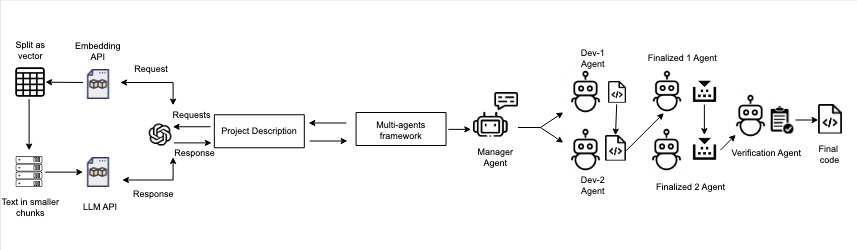
\includegraphics[width=1\linewidth]{images/CodePoriSchema.jpeg}
    \caption{Diagramme du workflow d'un système multi agent dirigé par IA pour la génération automatique de code \parencite{rasheed_codepori_2024}}
    \label{fig:schemaCodePori}
\end{figure}

\textbf{Évaluation.}
\begin{itemize}
  \item \textbf{Benchmark HumanEval} : 89\% de précision au test \textbf{Pass@1} (évaluant le taux de réussite au premier coup), surpassant plusieurs modèles de référence comme MetaGPT ou encore ChatDev.
  \item \textbf{Test manuel} sur 20 descriptions de projets : 85\% de code exécutable sans modifications (17 résultats concluants).
  \item \textbf{Coût et latence} : génération d’un projet complet "en quelques minutes" pour "quelques dollars"\footnote{Par exemple, pour un projet de détection de masque (visible sur la figure \ref{fig:projetsCodePori}) sur le visage, on a : 18 minutes pour 399 lignes de code et un coût de 1.02\$}. \cite{rasheed_codepori_2024}.
\end{itemize}

% rasheed_codepori_2024
% Our findings indicate that the proposed system is capable of generating accurate code for large and complex software projects within a few minutes.
% CodePori is able to generate running code for large-scale projects, aligned with the typical software development process within minutes, and at a cost of a few dollars.
%

\begin{figure}[H]
    \centering
    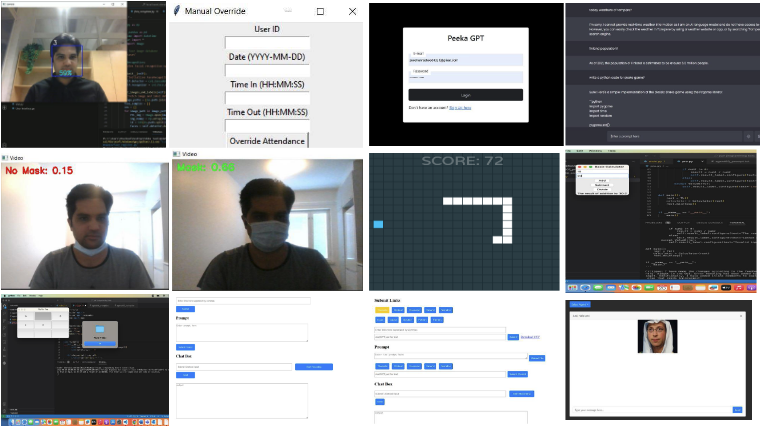
\includegraphics[width=0.75\linewidth]{images/CodePoriProjects.png}
    \caption{Logiciels développés par CodePori \parencite{rasheed_codepori_2024}}
    \label{fig:projetsCodePori}
\end{figure}

\paragraph{Forces et limites.}
CodePori démontre la faisabilité d’une équipe IA couvrant tout le cycle de développement (analyse → codage → tests → assurance qualité), mais l’étude souligne la dépendance à l’orchestration centrale et la nécessité d’itérations multiples pour obtenir un code pleinement fonctionnel.

\section{Cas d’étude : Agent-Driven Automatic Software Improvement}

\textcite{vallecillos_ruiz_agent-driven_2024} présente un projet doctoral qui vise à améliorer la maintenance logicielle en combinant \textbf{LLMs} et \textbf{agents IA} dans un cadre itératif de génération–révision.

\paragraph{Concept et architecture.}
La figure \ref{fig:schemaVallecillos} introduit un framework conceptuel composé d’un Agent LLM (Agent IA) et d’un critique (humain, outil ou autre LLM) échangeant sur des boucles continues pour affiner le code généré en donnant un retour entre chaque sortie (Output).  
\begin{figure}[H]
    \centering
    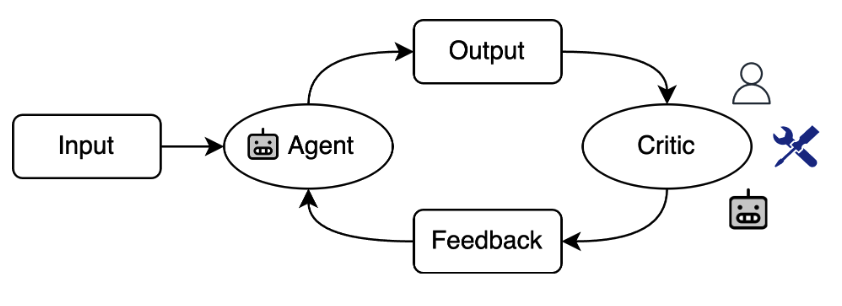
\includegraphics[width=0.75\linewidth]{images/VallecillosSchema.png}
    \caption{Framework conceptuel pour un Agent IA, \parencite{vallecillos_ruiz_agent-driven_2024}}
    \label{fig:schemaVallecillos}
\end{figure}

Trois scénarios d’interaction sont distingués (figure \ref{fig:schema2Vallecillos}) :  
\begin{enumerate}
  \item \textbf{Agent unique} agissant en autocontrôle;
  \item \textbf{Agents multiples} coopérant ou se spécialisant;
  \item \textbf{Human-in-the-loop} combinant expertise humaine et puissance de l’agent.
\end{enumerate}

\begin{figure}[H]
    \centering
    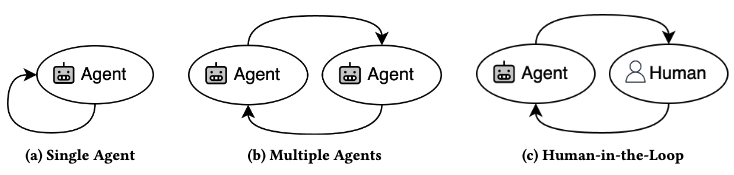
\includegraphics[width=0.75\linewidth]{images/VallecillosSchema2.png}
    \caption{Scenarios d’interactions entre Agents IA, \parencite{vallecillos_ruiz_agent-driven_2024}}
    \label{fig:schema2Vallecillos}
\end{figure}

\paragraph{Objectifs et contributions attendues.}
Le projet se déploie en trois phases correspondant aux questions de recherche :  
\begin{itemize}
  \item \textbf{RQ1} : comparer agent unique vs. usage one-shot d’un LLM sur des tâches d’amélioration de code;
  \item \textbf{RQ2} : étudier l’effet synergique d’équipes multi-agents spécialisées pour des scénarios complexes;
  \item \textbf{RQ3} : proposer de nouvelles méthodes de \emph{fine-tuning} tirant parti du processus itératif.
\end{itemize}

\paragraph{Boucles itératives et \emph{last-mile} problems.}
Les agents itératifs sont conçus pour résoudre les \textit{last-mile errors}, c’est-à-dire les bogues subtils apparaissant en toute fin de génération fonctionnelle. Chaque cycle d’itération permet :
\begin{enumerate}
  \item de recevoir un retour du critic ;
  \item de régénérer ou patcher la portion fautive ;
  \item d’améliorer progressivement sécurité, efficacité et style.
\end{enumerate}

\paragraph{Positionnement par rapport à l’état de l’art.}
L’auteur souligne que les approches mono-shot échouent souvent sur des codes complexes ou vulnérables, alors que des agents multi-itératifs sont plus compétents et plus aptes, par exemple, à régler un "last-mile problem".

\paragraph{Forces et limites.}
\begin{itemize}
  \item \textbf{Forces :} cadre générique, possibilité d’exploiter des experts spécialisés, amélioration continue via feedback loops.
  \item \textbf{Limites :} orchestration complexe, besoin d’une comparaison systématique des approches multi-agent, dépendance aux coûts d’appels API et à la qualité des critiques.
\end{itemize}

\section{Autres frameworks récents}

\subsection{Pipelines Auto-DevOps multi-agents}

\textcite{khan_ai-driven_2025} décrivent un cadre multi-agent intégré aux pratiques DevOps :  
des agents LLM distincts s’occupent de la planification de sprint, de la génération de code, de l’exécution automatique de tests et du déclenchement de pipelines CI/CD.  
Les auteurs rapportent une réduction du temps de développement et une meilleure cohérence entre le backlog et le code livré grâce à la distribution dynamique des tâches et au feedback continu entre agents.
% khan_ai-driven_2025
% Our study demonstrates that AI-driven automation can enhance various stages of the  software development lifecycle, including sprint planning, code generation, bug detection, and  testing. By leveraging specialized AI agents that collaborate dynamically, development teams can  streamline workflows, reduce errors, and accelerate project timelines.
%

\subsection{Retours d’expérience industriels ou open-source}

Dans un contexte industriel, \textcite{abbas_ai-driven_2024} montrent qu’une adoption progressive d’agents LLM pour la revue de code, la priorisation du backlog et l’automatisation des tests permet d’alléger la charge des développeurs et d’augmenter la productivité globale des équipes.  
Les agents interviennent notamment pour :
\begin{itemize}
  \item générer la documentation et détecter les risques en temps réel ;
  \item automatiser la revue de code et proposer des correctifs.
\end{itemize}

\section{Évaluation empirique}

La comparaison des prototypes et retours d'expérience fait ressortir trois indicateurs récurrents :

\begin{itemize}
  \item \textbf{Réduction du temps de développement} : les pipelines multi-agents permettent d’accélérer la planification et l’intégration continue \parencite{khan_ai-driven_2025}.
  \item \textbf{Amélioration de la productivité et de la détection d’erreurs} : l’automatisation des tâches répétitives (documentation, tests, revue) libère du temps pour les activités à forte valeur ajoutée \parencite{abbas_ai-driven_2024}.
  \item \textbf{Cohérence backlog $\leftrightarrow$ code livré} : la coordination d’agents spécialisés assure une meilleure traçabilité des exigences fonctionnelles jusqu’au code \parencite{khan_ai-driven_2025}.
\end{itemize}


%%%%%%%%%%%%%%%%%%%%%%%%%%%%%%%%%%%%%%%%%%%%%%%%%%%%%%%%%%%%%%%%%%%%%%%

% ========================
% ==== Evaluation faisabilite 
% ========================

\chapter{Faisabilité et perspectives du remplacement total} \label{chapitre:faisabilite}

\section{Cartographie des tâches d’une équipe de développement}

Les articles de notre bibliographie font apparaître un ensemble récurrent de \textbf{huit fonctions} que toute équipe de développement — humaine ou multi-agents — doit couvrir :

\begin{itemize}
  \item \textbf{Analyse des exigences \& priorisation du backlog} \parencite{ashraf_autonomous_2025, abbas_ai-driven_2024}.
  \item \textbf{Planification de sprint \& management de projet} \parencite{khan_ai-driven_2025}.
  \item \textbf{Génération et refactorisation du code} \parencite{rasheed_codepori_2024, zahid_multi-agent_2024}.
  \item \textbf{Tests automatisés et validation fonctionnelle} \parencite{rasheed_codepori_2024, khan_ai-driven_2025}.
  \item \textbf{Débogage et correction de bugs} \parencite{ashraf_autonomous_2025, vallecillos_ruiz_agent-driven_2024}.
  \item \textbf{Documentation et génération de rapports} \parencite{ashraf_autonomous_2025, zahid_multi-agent_2024}.
  \item \textbf{Revue de code / Assurance qualité} \parencite{rasheed_codepori_2024, abbas_ai-driven_2024}.
  \item \textbf{Intégration \& déploiement continus (CI/CD)} \parencite{khan_ai-driven_2025}.
\end{itemize}


\section{Couverture actuelle par les agents IA}

Les études analysées montrent un niveau d’automatisation contrasté :  
\begin{itemize}
  \item \textbf{Développement :} fort (85 à 89\% de précision HumanEval avec CodePori) \parencite{rasheed_codepori_2024}.  
  \item \textbf{Refactorisation / bug fixing :} amélioration notable via pipelines itératifs \parencite{vallecillos_ruiz_agent-driven_2024}.  
  \item \textbf{Tests générés automatiquement :} partiel, dépend de la couverture de benchmarks \parencite{abbas_ai-driven_2024}.  
  \item \textbf{Architecture et priorisation produit :} faible ; décisions stratégiques requièrent toujours une validation humaine \parencite{handler_taxonomy_2023}.  
  \item \textbf{DevOps :} automatisation des pipelines CI/CD prometteuse mais encore supervisée \parencite{khan_ai-driven_2025}.
\end{itemize}

\section{Analyse SWOT d’une équipe 100 \% IA}

Avant de statuer sur la faisabilité d’un remplacement total, il est utile de synthétiser, sous forme SWOT, les \textbf{forces} (Strength), \textbf{faiblesses} (Weaknesses), \textbf{opportunités} (Opportunities) et \textbf{menaces} (Threats) dégagées par les études de cas et simulations précédentes.  
Le tableau \ref{tab:SWOT} résume ces facteurs :

\begin{table}[H]
    \begin{tabular}{|p{2.5cm}|p{6cm}|p{6cm}|}
        \hline
        \textbf{Strength} & Vitesse d'exécution quasi 24/7 \parencite{ashraf_autonomous_2025} & Réduction des coûts unitaires \parencite{rasheed_codepori_2024} \\
        \hline
        \textbf{Weaknesses} & Hallucinations, biais, dettes techniques \parencite{cui_risk_2024} & Dépendance aux API propriétaires \parencite{rasheed_codepori_2024}\\
        \hline
        \textbf{Opportunities} & Nouveaux modèles SaaS sans humains & Personnalisation rapide pour marchés verticaux \\
        \hline
        \textbf{Threats} & Fuite de données / attaques back-door \parencite{wang_unique_2024} & Éthique et responsabilité légale \\
        \hline
    \end{tabular}
    \caption{Analyse SWOT d'une équipe 100\% IA}
    \label{tab:SWOT}
\end{table}

\section{Scénarios d’évolution}

Les retours d’expérience et prototypes étudiés suggèrent une trajectoire en trois paliers pour l’adoption des agents IA dans le développement logiciel.

\subsection{Court terme : collaboration homme–IA}

Dans la phase actuelle, les agents agissent avant tout en supplément, comme co-pilotes :  
\begin{itemize}
  \item génération ou complétion de code, recherche de snippets, écriture de tests unitaires ;
  \item suggestions de refactorisation et détection précoce de failles courantes.  
\end{itemize}
Le développeur reste le \textbf{reviewer critique}, relit et valide chaque changement avant fusion.  
\textcite{zahid_multi-agent_2024} soulignent que malgré les capacités des agents en terme de détection de bug, l'intervention humaine reste essentielle pour gérer des problèmes complexes et fortement contextualisés.

\subsection{Moyen terme : équipes hybrides réduites}

Dans une équipe hybride, on pourrait viser un ratio d'un humain pour cinq agents IA, l’humain restant responsable de l’architecture et de la validation métier.
 
L’humain se concentrerait sur :
\begin{itemize}
  \item la définition de l’architecture / des priorités produit ;
  \item l’arbitrage des décisions critiques (sécurité, budget).  
  \item éventuellement la relecture avant déploiement
\end{itemize}
Les agents IA, orchestrés dans un workflow continu, prennent en charge :
\begin{enumerate}
  \item le codage et la documentation ;
  \item l’exécution automatique de tests et le débogage ;
  \item la mise à jour des pipelines CI/CD et du monitoring.  
\end{enumerate}
\textcite{khan_ai-driven_2025} rapportent que cette configuration réduit le temps de développement tout en maintenant un feedback loop humain aux points de contrôle clés (déploiement, ...).

\subsection{Long terme : autonomie complète sous supervision minimale}

À horizon plus lointain, on peut envisager une \textbf{équipe 100 \% IA} livrant en continu, avec :
\begin{itemize}
  \item un contrôle a posteriori : audits périodiques et tests de conformité ;  
  \item des guardrails de sûreté (policies, sandboxing) pour limiter les dérives \parencite{cui_risk_2024}.  
\end{itemize}
Les tâches humaines se déplacent vers :
\begin{itemize}
  \item la gouvernance (définition d’objectifs, gestion des risques) ;  
  \item la validation légale et réglementaire ;  
  \item l’optimisation des coûts d’infrastructure LLM et la mise à jour des modèles.  
\end{itemize}
Ce scénario demeure conditionné à la résolution des menaces identifiées : fuites de données et attaques backdoor \parencite{wang_unique_2024}, ainsi qu’à l’instauration d’un cadre de responsabilité clair pour les décisions prises par les agents.

\paragraph{Ouverture éthique}Ces perspectives soulèvent néanmoins une question fondamentale : \textit{remplacer entièrement les développeurs humains par des agents IA serait-il éthique, juste et socialement acceptable ?}


%%%%%%%%%%%%%%%%%%%%%%%%%%%%%%%%%%%%%%%%%%%%%%%%%%%%%%%%%%%%%%%%%%%%%%%

% ========================
% ==== Conclusion
% ========================

\chapter{Conclusion} \label{conclusion}

Ce mémoire est parti d’une interrogation simple : l’automatisation par agents IA peut-elle aller jusqu’à remplacer entièrement une équipe de développement ?
Pour y répondre, nous avons d’abord parcouru l’état de l’art des LLMs, décrit les architectures multi-agents et analysé trois prototypes — CodePori (89 \% de réussite sur HumanEval), le cadre itératif Agent-Driven Automatic Software Improvement, et les pipelines Auto-DevOps présentés par \textcite{khan_ai-driven_2025}. Ces études de cas montrent qu’une grande partie des tâches techniques — génération, tests, documentation ou débogage — est déjà couverte avec un niveau de fiabilité oscillant entre 80\% et 90\% de précision.

L’examen systématique des fonctions clés d’une équipe (de l’analyse d’exigences à la mise en production) révèle toutefois que deux domaines échappent encore largement à l’autonomie : la définition stratégique du produit et la gouvernance qualité. Les agents sont rapides : ils livrent du code exécutable en quelques minutes pour quelques dollars \parencite{rasheed_codepori_2024}, mais demeurent vulnérables aux hallucinations et aux biais \parencite{cui_risk_2024}, ainsi qu’aux attaques de type backdoor ou fuite de données \parencite{wang_unique_2024}. Tant que ces risques ne sont pas entièrement maîtrisés, une supervision humaine reste indispensable, au moins a posteriori, pour valider les livraisons et assumer la responsabilité légale.

Notre analyse conduit donc à une réponse nuancée. Oui, le remplacement total est envisageable sur le plan technique ; non, il n’est pas encore acceptable sans trois garanties :

\begin{itemize}
    \item un dispositif d’alignement solide (guardrails, traçabilité),
    \item une gestion rigoureuse de la sécurité et de la confidentialité,
    \item un cadre de gouvernance qui précise qui ou quoi porte la responsabilité des choix d’architecture, de budget et de conformité
\end{itemize}

En proposant une cartographie fonctionnelle, une synthèse critique des prototypes et une matrice SWOT, ce travail apporte un panorama structuré des points de bascule où l’IA devance déjà l’humain, et des verrous qui subsistent. Ses limites résident principalement dans la rareté de données industrielles ouvertes et l’incertitude sur les coûts d’inférence à grande échelle. Les perspectives logiques sont doubles : d’un côté, la création de benchmarks plus représentatifs (intégrant dette technique et sécurité), de l’autre, l’étude des impacts organisationnels et éthiques d’équipes entièrement IA.

En définitive, la question n’est plus tant "peut-on" automatiser, mais plutôt dans quelles conditions et avec quelles garanties nous choisirons (ou non) de le faire.

%%%%%%%%%%%%%%%%%%%%%%%%%%%%%%%%%%%%%%%%%%%%%%%%%%%%%%%%%%%%%%%%%%%%%%%

% ========================
% ==== Bibliograpghie 
% ========================

\printbibliography[%
    nottype=online,
    title={Bibliographie},  % titre personnalisé
    heading=bibintoc        % ajoute au TOC comme chapter
]

%%%%%%%%%%%%%%%%%%%%%%%%%%%%%%%%%%%%%%%%%%%%%%%%%%%%%%%%%%%%%%%%%%%%%%%

% ========================
% ==== Webographie
% ========================

\printbibliography[
  type=online,
  title={Webographie},
  heading=bibintoc
]

%%%%%%%%%%%%%%%%%%%%%%%%%%%%%%%%%%%%%%%%%%%%%%%%%%%%%%%%%%%%%%%%%%%%%%%

% ========================
% ==== Annexe
% ========================

\chapter{Annexes}
\appendix
\makeatletter
\def\@seccntformat#1{Annexe~\csname the#1\endcsname:\quad}
\makeatother

\section{Mots éliminatoires pour les titres}\label{annexe:mots_eliminatoires}
Afin de garantir la pertinence des articles retenus, les titres comportant l’un des mots suivants sont exclus :
\begin{lstlisting}[breaklines=true,basicstyle=\ttfamily\small]
ELIMINATORY_WORDS = ["philosophy","sociology","ethics","political","policy","society","healthcare","clinical","gender","history","art","religion","linguistics","psychology"]
\end{lstlisting}


%%%%%%%%%%%%%%%%%%%%%%%%%%%%%%%%%%%%%%%%%%%%%%%%%%%%%%%%%%%%%%%%%%%%%%%

\newpage
\thispagestyle{empty} % pas de numéro de page
\null               % boîte vide pour générer la page

\end{document}